\par
We used the data-taking periods from 2010 LHC operations 
passing the standard CMS quality criteria, which allow no anomalous or
faulty behavior for the inner tracker, the calorimeters,
and the muon chambers.
\par
Several large samples of simulated events were used to evaluate the signal
and background efficiencies and to validate our analysis techniques.
Samples of electroweak processes with $\Wo$ and $\Zo$ production, both for
signal and background events, were produced with
POWHEG~\cite{Alioli:2008gx, Nason:2004rx, Frixione:2007vw},
interfaced with the PYTHIA~\cite{Sjostrand:2006za} parton-shower generator.
QCD events with muons, electrons, or jets likely to be misidentified
as electrons in the final state were studied with PYTHIA, as were other minor
backgrounds such as $\ttbar$ and certain electroweak processes
($\Wtn$, $\Ztt$, $\Wo\Wo$, $\Wo\Zo$, and $\Zo\Zo$).
We do not consider the diboson channels ($\Wo\Wo$, $\Wo\Zo$, and $\Zo\Zo$)
as part of the $\Wo$ and $\Zo$ signals in order to facilitate the comparison 
of our results to theoretical predictions,
which do not take these contributions into account.
Generated events were processed through the full GEANT4~\cite{GEANT4} detector 
simulation, trigger emulation, and event reconstruction chain.

\subsection{$\Wo$ boson selection}

\par
The $\Wo$ events are characterized by a prompt, energetic, and
isolated lepton, and significant missing energy.
The main backgrounds are QCD multijet events and Drell-Yan (DY)
events in which one lepton fails the selection.  The QCD background is
reduced by requiring the lepton to be isolated; the remaining
events do not have large $\MET$ and can be distinguished from
signal events on a statistical basis.  The DY background
is suppressed by rejecting events with a second lepton candidate.

To measure the signal yields, we choose to fit the $\MET$
distribution for both the electron and muon channels.
According to the simulation, $\Wtn$ background contribution is small,
while backgrounds from $\Ztt$, $\ttbar$, and diboson production
are negligible in both electron and muon channels.

\subsection{$\Wen$ signal extraction\label{sec:Wen}}

The $\Wen$ candidate events are required to have one identified electron
with an ECAL cluster of $\et > 25\GeV$ in the ECAL fiducial volume.
If a second electron candidate
satisfying looser criteria and with $\et > 20\GeV$ is present in
the event, the event is rejected.
%The fraction of signal events selected in the simulation is
%$\APRIM{\Wo} = \WEIAPRIM$, with  $\APRIM{\Wop}=\WEPAPRIM$ and
%$\APRIM{\Wom}=\WEMAPRIM$.
The number of events selected in the data
is $\WEISAMPLE$, with $\WEPSAMPLE$ positive and $\WEMSAMPLE$
negative electrons.
\par
The $\Wen$ signal is extracted from an unbinned maximum likelihood
fit of the observed $\MET$ distribution to the sum of signal and
background shapes.
The QCD background shape, which accounts
for both QCD multijet production and direct-photon
production with the photon converting in the detector,
can be modeled by a modified Rayleigh distribution,
$$f(\MET) = \MET \times \exp{\left(-\frac{\MET^2}{2(\sigma_0+\sigma_1\MET)^2}\right)}.$$
This function can be understood as describing fluctuations of the
missing transverse momentum vector around zero due to measurement errors;
%the resolution term, $\sigma_0+\sigma_1 \MET$, increases
%with $\MET$ to account for tails in the $\MET$ measurement.  
%This function describes well the QCD background shape in the simulation, over the full
%range of $\MET$, as well as $\MET$ distributions from signal-free samples obtained by 
%inverting the identification or isolation criteria.
The fit to the anti-selected sample shown on
Fig.~\ref{fig:e-inverted} illustrates the quality of the description
of the background shape by our parameterized function,
including in the region of the signal, at high \MET.
\begin{figure}[b]
\begin{center}
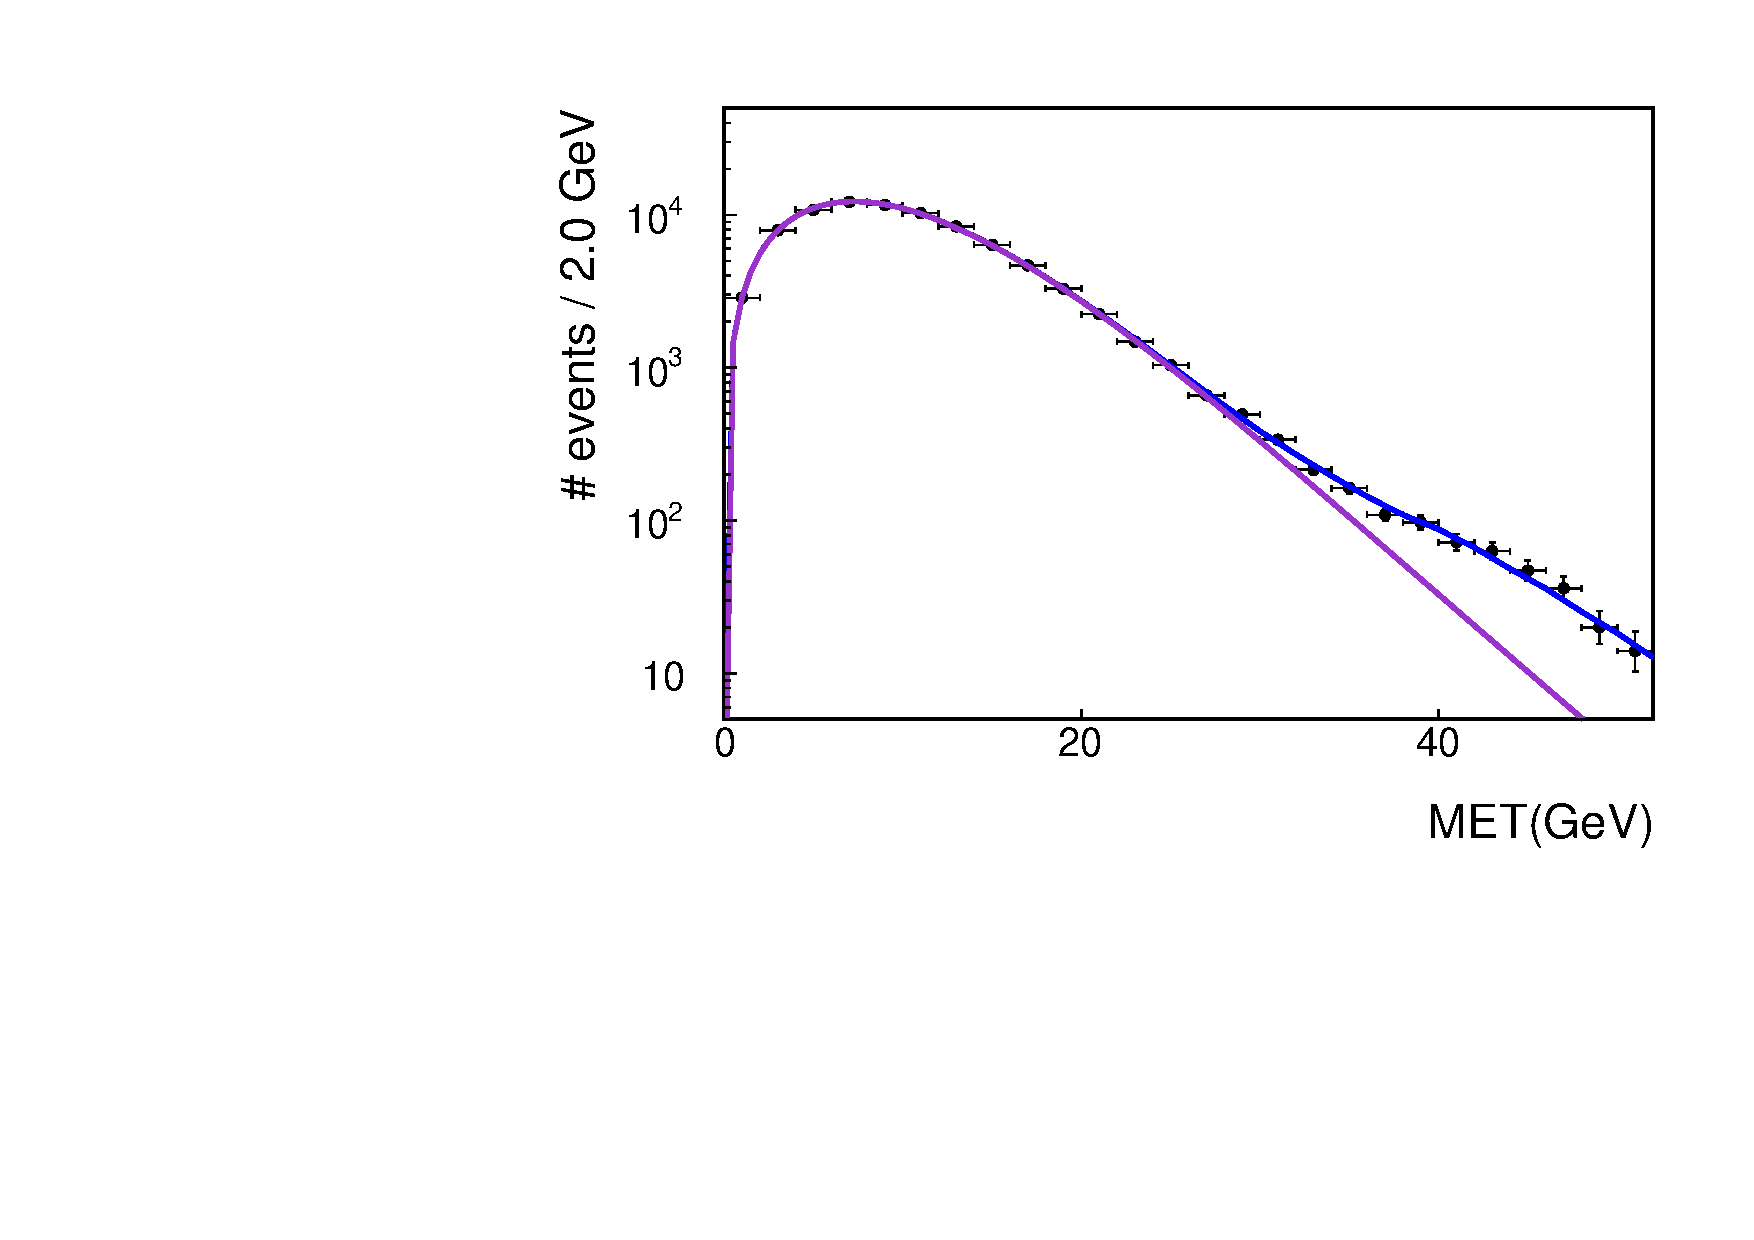
\includegraphics[width=0.50\textwidth]{figs/fixedMCyield_normal_model.pdf}
\caption{Fit to the anti-selected background sample (we invert cuts on the track-match
variables while maintaining the usual \ET and ECAL-iso selections).
}\label{fig:e-inverted}
\end{center}
\end{figure}


The signal distributions are derived from simulation,
separately for $\Wp$ and $\Wm$, and receive
an event-by-event correction in bins of the $\Wo$ transverse momentum,
determined from a study of the hadronic recoil
distributions of $\Zee$ events in the data.%~\cite{CMS-PAS-JME-10-005}.
In fig.~\ref{fig:Recoil} the left-hand side plot demonstrates the effect of the recoil
corrections on the MET shape for the electron channel while the right-hand side plot
shows the uncertainty from the recoil method propagated to the corrected W MET shape.


%%%%%%%%%%%%%%%%%%%%%%%%%
\begin{figure}
\begin{center}
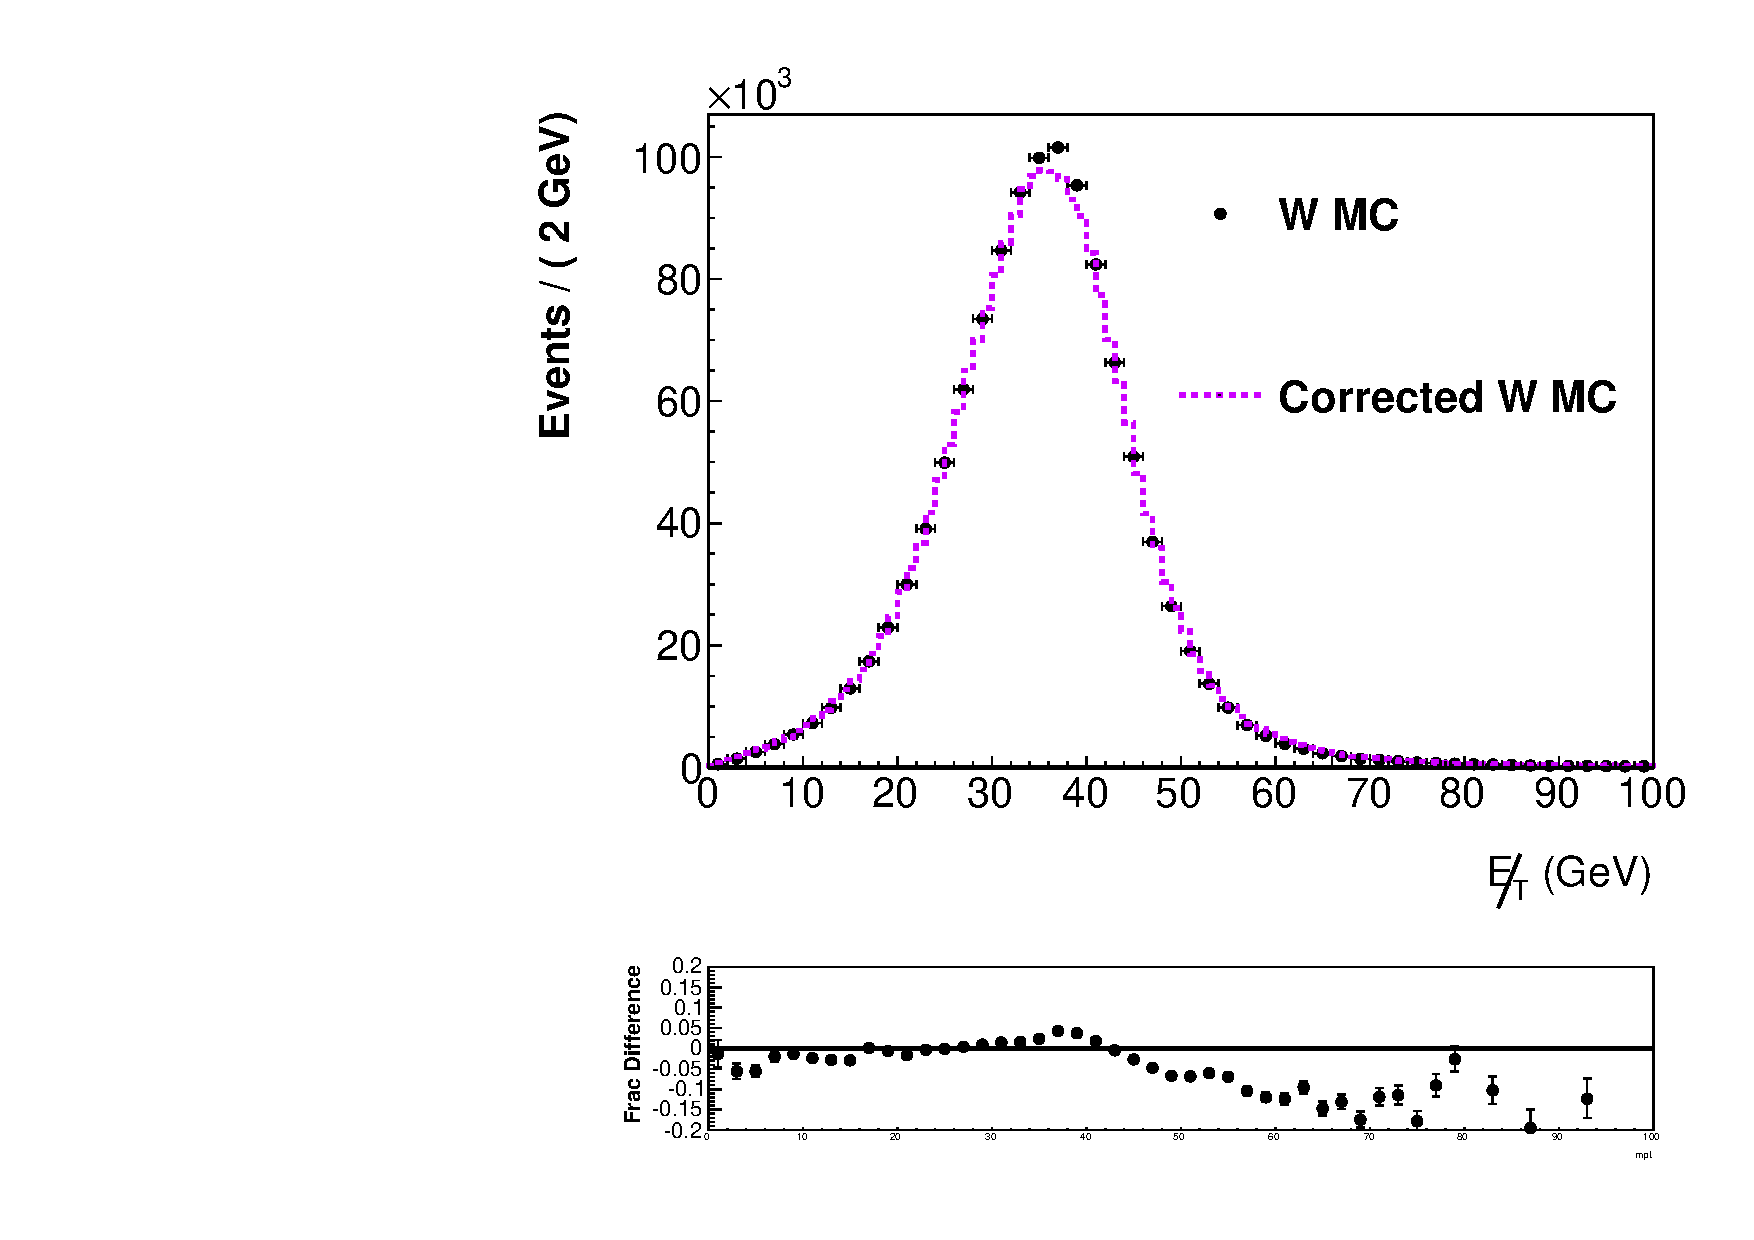
\includegraphics[width=0.48\textwidth]{figs/beforeANDafter.pdf}
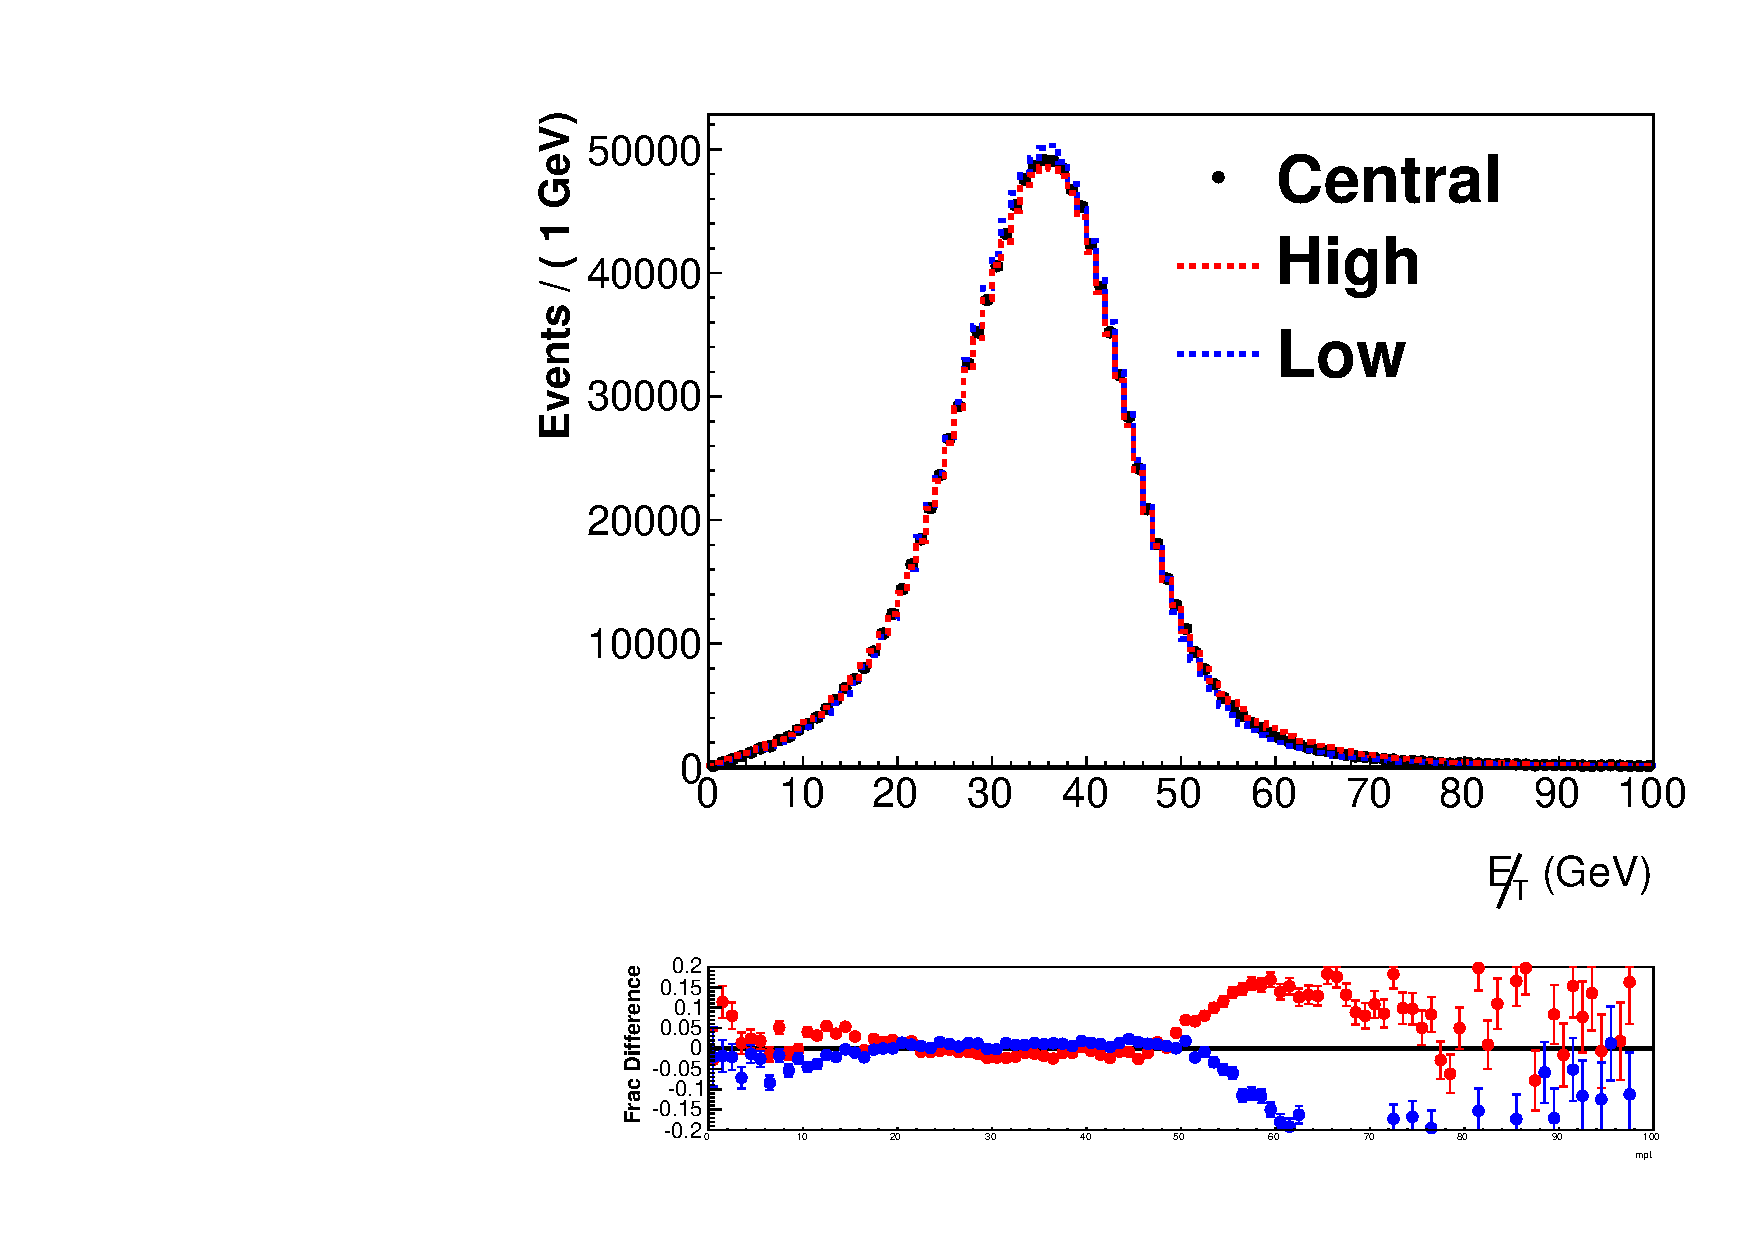
\includegraphics[width=0.48\textwidth]{figs/upANDdown.pdf}
\caption{ \label{fig:Recoil}
Demonstration of the recoil corrections on the $\Wen$ $\MET$ shape (left)
and uncertainties from the recoil method propagated to the corrected
$\Wen$ $\MET$ shape (right).
}
\end{center}
\end{figure}
%%%%%%%%%%%%%%%%%%%%%%%%%


%In fits to the $\MET$ distributions, the free parameters
%are the $\Wo$ signal yield, the QCD background yield, and
%the shape parameters $\sigma_0$ and $\sigma_1$.

We extract the inclusive yield $\NSIG{\Wo}$ from a fit where
the expected ratio for $\XVL{\sigma}{(\Wp)}/\XVL{\sigma}{(\Wm)}$
is assumed.
It has been  checked that the result was insensitive to this assumption.
Figure~\ref{fig:Wenu}~(a) shows the $\MET$ distribution of
the inclusive $\Wen$ sample
and the results of the likelihood fit.
%the fit function describes the
%data well, with a $p$-value of $\WEIKSPCOR$ for the Kolmogorov-Smirnov test.
The inclusive yield is $\NSIG{\Wo} = \WEIYIELD$ events.

%%%%%%%%%%%%%%%%%%%%%%%%%
\begin{figure}[t]
\begin{center}
         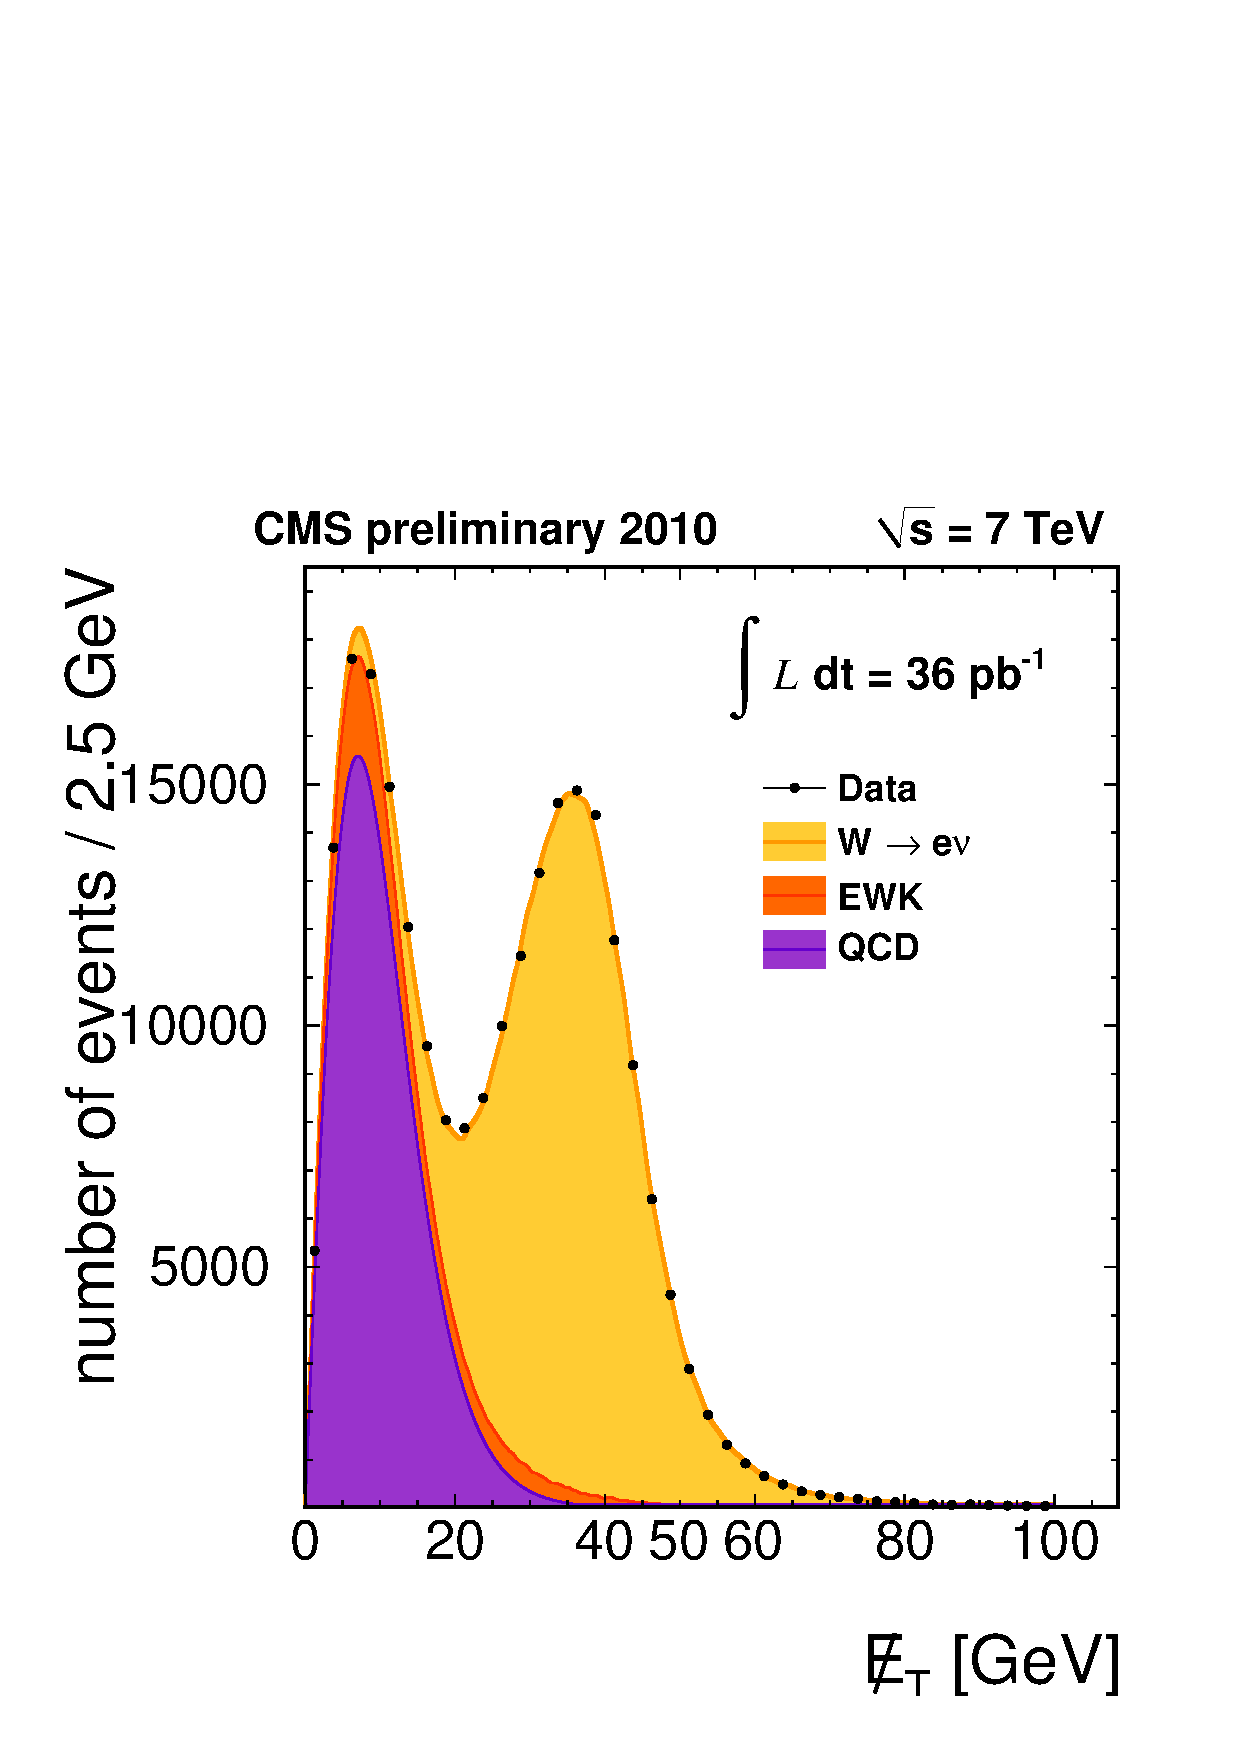
\includegraphics[width=.45\textwidth]{figs/w_inc_36pb.pdf}
        \hspace{.05in}
         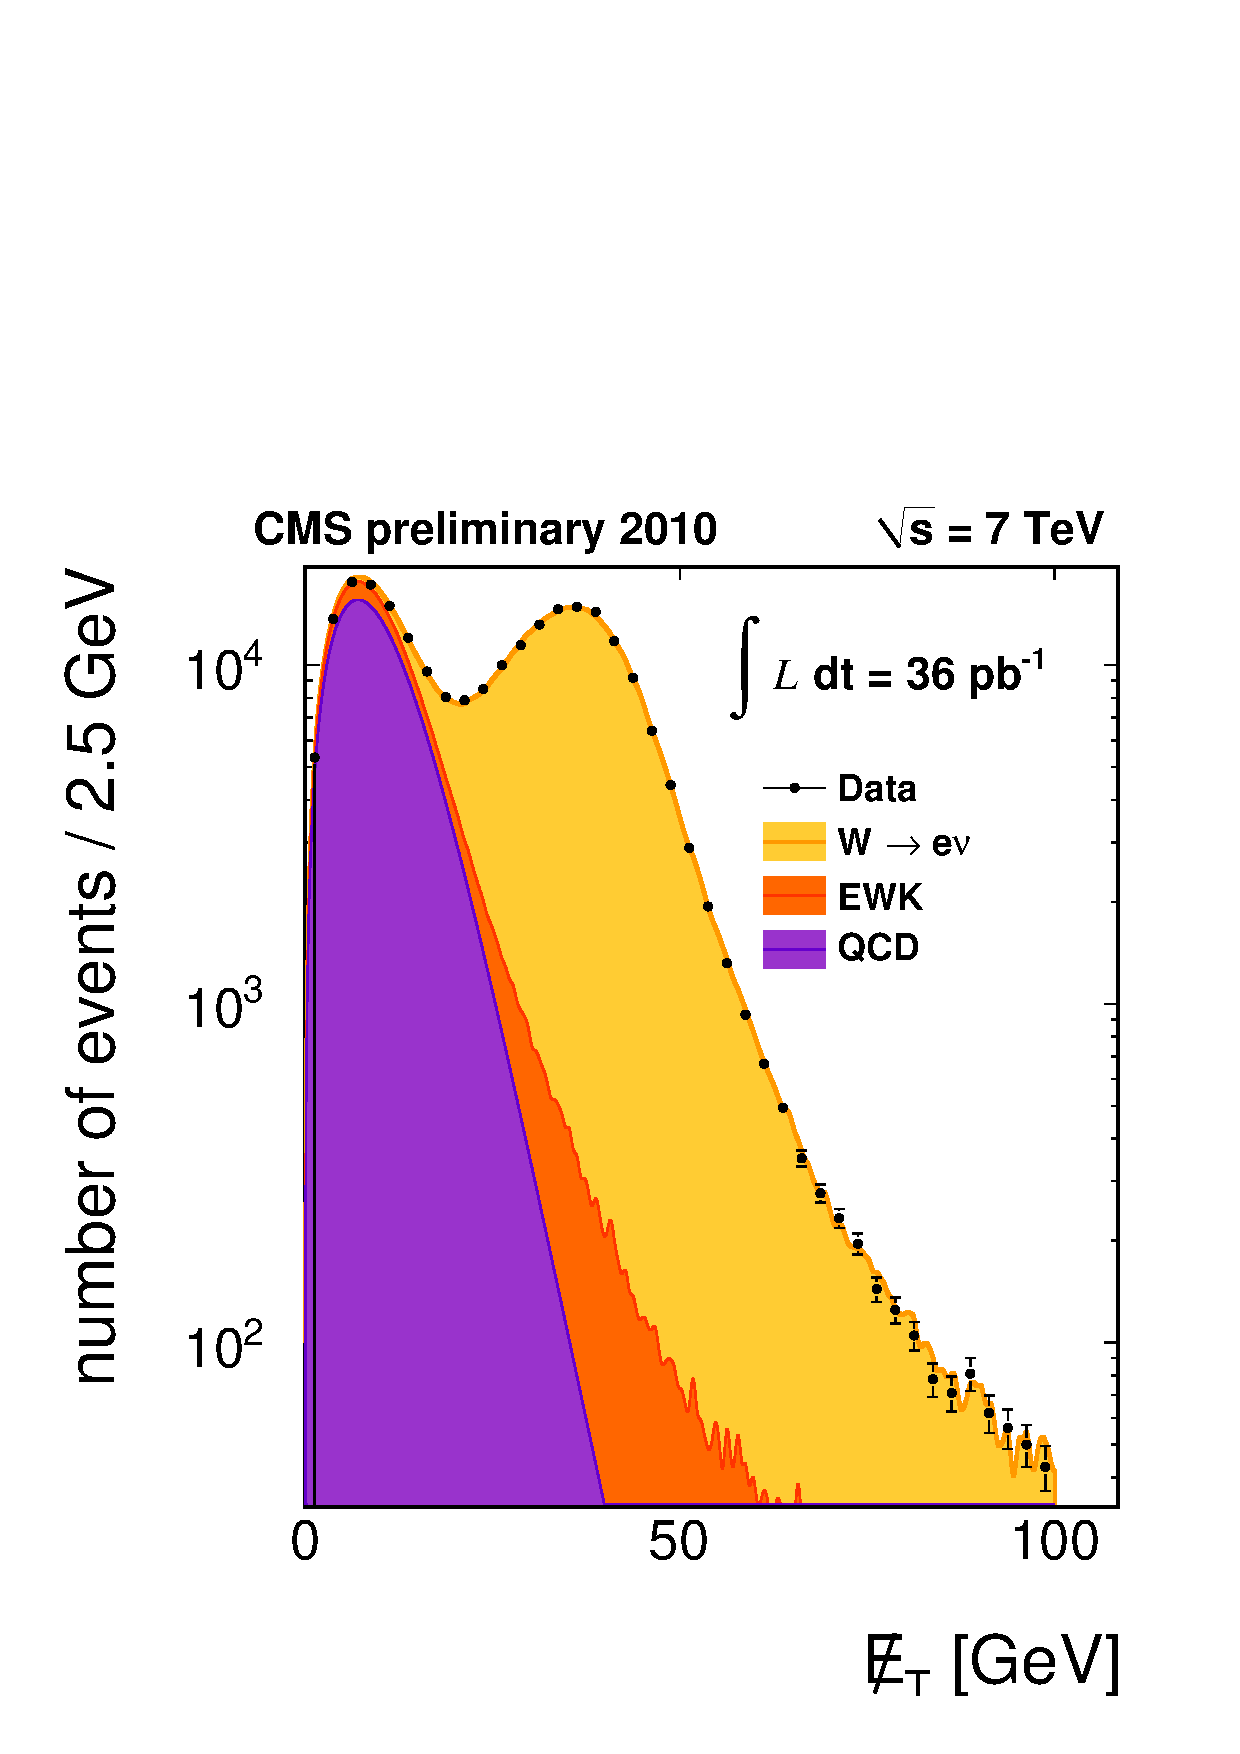
\includegraphics[width=.45\textwidth]{figs/w_inc_36pb_log.pdf}
        \hspace{.05in}
       \caption{The $\MET$ distributions for the $\Wen$ candidates:~(a)
linear scale;~(b)~log-scale.  The points represent
the data.  Superimposed are the results of the maximum likelihood fits for
signal plus backgrounds, in yellow; all backgrounds, in orange;
QCD backgrounds, in violet.
\label{fig:Wenu} }
\end{center}
\end{figure}
%%%%%%%%%%%%%%%%%%%%%%%%%


The signals for the $\Wpen$ and $\Wmen$ channels are
extracted from a simultaneous fit to the individual $\MET$
distributions, in which the QCD background  shape parameters $\sigma_0$ and
$\sigma_1$ are constrained to be the same for both samples.
The yields are $\WEPYIELD$ for $\Wpen$ and $\WEMYIELD$
for $\Wmen$, with a negligible correlation.
%Because the two fits are independent,
%the relation $\NSIG{\Wo} = \NSIG{\Wop} + \NSIG{\Wom}$ is not exactly satisfied,
%but holds to within 0.2\%.

Two additional signal extraction techniques were explored. 

In the first approach the QCD \MET template is extracted directly from the data using a
control sample obtained by inverting a subset of the cuts used to select the
signal. In this way, the shape of the template is fixed from the data, and
only the normalization is allowed to float in the fit. 
%The advantage of this approach
%is that detector effects such as anomalous signals in the calorimeters, or
%dead ECAL towers, are automatically reproduced in the QCD template, since these
%effects are not affected by the cut inversion used to define the control sample.
Possible differences in shape between the selected and anti-selected \MET
distributions has been found to be due to a combination of two effects,
and can be eliminated by applying corrections.  In the
Particle Flow algorithm, electron candidates contribute differently to
\MET depending on the output of a multivariate analysis (MVA) used to identify
electrons.  A correction is applied to account for the fact that the
distribution of the MVA output is very different in the signal and
control samples, resulting in a bias to the \MET shape.  The second
correction accounts for the effect of a small observed correlation between
one of the inverted variables and \MET.  The correction is derived by performing linear
fits, separately for the ECAL barrel and endcaps, to profile histograms of
the mean value of \MET in slices of the inverted variable.


The results of inclusive fits for \MET and $M_T$ using the fixed shape QCD
template are shown in Figure~\ref{fig:resultAll}.

\begin{figure}[htb]
  \begin{center}
    \includegraphics*[width=0.9\textwidth]{figs/resultsAll.pdf}
    \caption{Result of fixed shape template fits for \MET (left) and $M_T$
(right) for all W candidates.  The bottom plots show the ratio of the data to
the sum of the fitted templates.}
    \label{fig:resultAll}
  \end{center}
\end{figure}

%By applying the method we obtain the following yields:
% 134894 $\pm$ 384 for the inclusive sample, xx $\pm$ xx for $\Wpen$ sample and
% xx $\pm$ xx for $\Wmen$ sample. Those yields are in good agreement with the
% parametrized fits method.

By applying the method we obtain a yield of 134894 $\pm$ 384 (stat) for the inclusive sample. 
The ratio of the inclusive yields between this method and the parameterized QCD shape is
0.989 $\pm$ 0.005 considering only the uncorrelated systematics between the two methods. 

In the second approach the data are divided into 5 categories defined by cuts 
on $\MET$ and relative tracker isolation of the electron candidate.
The ABCD region in this method roughly maps onto the AB region of the older approach, 
with the E box mapping onto the CD region. This particular arrangement is chosen to minimize 
the sensitivity to uncertainties on the background model. A system of equations is constructed 
relating the number of observed data events in each of the four regions to the number of 
background and signal events, with a number of parameters to be determined from auxilliary 
measurements or simulations. By applying the method we obtain the following yields:
135858 $\pm$ 496 (stat) for the inclusive sample, 81407 $\pm$ 384 (stat) for $\Wpen$ sample and
54319 $\pm$ 315 (stat) for $\Wmen$ sample, with negligible correlation.
The ratio of the inclusive yields between this method and the parameterized QCD shape is
0.997 $\pm$ 0.007 considering only the uncorrelated systematics between the two methods. 

The EWK backgrouds consist mainly of $\Zee+\Ztt$ (7.6$\%$), $\Wtn$ (3.0$\%$), 
di-bosons (0.14$\%$) and $\ttbar$ (0.44$\%$).

